\documentclass{article}
\usepackage{graphicx} % Required for inserting images
\usepackage{graphicx} % Required for inserting images

\usepackage[utf8]{inputenc}
\usepackage[utf8]{inputenc}

\usepackage{times}
\usepackage[papersize={17cm,24cm},margin=22mm,top=17mm,headsep=5mm]{geometry}
\usepackage[dvipsnames]{xcolor}
\usepackage[english]{babel} % multilinguality

\definecolor{bred}{rgb}{0.8,0,0}
\usepackage{dsfont}
\usepackage{microtype}
\usepackage{graphicx}
\usepackage{subfigure}
\usepackage{booktabs} % for professional tables
\usepackage{amsfonts}
\usepackage{amsmath,amssymb,graphicx,epsfig}
\usepackage{enumerate,amsthm,epstopdf}

\usepackage[utf8]{inputenc} % allow utf-8 input
\usepackage[T1]{fontenc}    % use 8-bit T1 fonts


\usepackage{bbm}
\usepackage{xargs}
\usepackage{enumerate}
\usepackage{latexsym}
\usepackage{wasysym}
\usepackage{lineno}
\linenumbers
\usepackage{float}
\usepackage{hyperref}       % hyperlinks
\usepackage{url}            % simple URL typesetting
\usepackage{booktabs}       % professional-quality tables
\usepackage{amsfonts}       % blackboard math symbols
\usepackage{nicefrac}       % compact symbols for 1/2, etc.
\usepackage{microtype}      % microtypography
%\usepackage[square,numbers]{natbib}
%\usepackage{cleveref}
%\usepackage{eufrak}



\bibliographystyle{elsarticle-harv} 
%\usepackage{refcheck}
%\usepackage{showlabels}
\usepackage[textsize=footnotesize]{todonotes}

\definecolor{bred}{rgb}{0.8,0,0}

\hypersetup{colorlinks,linkcolor={blue},citecolor={bred},urlcolor={blue}}
\usepackage[textsize=footnotesize]{todonotes}
\newcommand{\tn}{\tilde{\theta}^\lambda_n}
\newcommand{\E}{\mathbb{E}}
\newcommand{\xtk}{x_{t,k}}
\newcommand{\ftk}{f_{t|k}}
\newcommand{\fkt}{f_{k|t}}
\newcommand{\hl}{h_\lambda}
\newcommand{\xk}{\tilde{x}_k}
\newcommand{\fk}{\tilde{f}_k}
\newcommand{\pt}{\hat{\pi}_t}
\newcommand{\pkl}{\hat{\pi}_{k\lambda}}
\newcommand{\Fkl}{F_{kl}}
\newcommand{\fin}{\phi^{-1}(z)}
\newcommand{\tH}{\Tilde{H}}
\newcommand{\ptk}{\hat{\pi}_{\theta_t|\theta_{k\lambda}}}
\newcommand{\acu}{{AC\cup U}}
\newcommand{\aref}[1]{$\mathbf{A}$\ref{#1}}
\newcommand{\bref}[1]{$\mathbf{C}$\ref{#1}}
\newcommand{\lref}[1]{$\mathbf{B}$\ref{#1}}
\newcommand{\rl}{r_\lambda}
\newcommand{\R}{R_\lambda}



\begin{document}
We are going to present a simple example where our algorithm is able to solve problems that are posed by a superlinear-growing gradient.
We use a stochastic gradient version of our algorithm to sample from $\pi_\beta=\frac{e^{-\beta u}}{\int_\mathbb{R}^d e^{-\beta u(x)}dx}$.
Knowing that this measure for large $\beta$ concentrates around the minimizer of $u$ the sampling algorithm can be used as an optimizer.
In this example, we set $d=1$. Consider the following optimization problem:
$$
\operatorname{minimize} \quad \mathbb{R} \ni \theta \mapsto u(\theta):=\mathbb{E}[U(\theta, X)],
$$
where $U: \mathbb{R} \times \mathbb{R} \rightarrow \mathbb{R}$ is defined by
$$
U(\theta, x)=\left\{\begin{array}{l}
a_1 \theta^2 \mathds{1}_{\{x \leq \theta\}}+a_2 \theta^2 \mathds{1}_{\{x>\theta\}}+\theta^{30}, \quad|\theta| \leq 1, \\
\left(a_3|\theta|+a_4\right) \mathds{1}_{\{x \leq \theta\}}+\left(a_5|\theta|+a_6\right) \mathds{1}_{\{x>\theta\}}+\theta^{30}, \quad|\theta|>1
\end{array}\right.
$$
with $a_3, a_4, a_5, a_6 \in \mathbb{R}$ satisfying
$$
a_3=2 a_1, \quad a_4=-a_1, \quad a_5=2 a_2, \quad a_6=-a_2
$$
for any fixed $a_1, a_2 \in \mathbb{R}$.
We run the experiment for $a_1=2$ $a_2=1$, $10^4$ iterations, with $\lambda=10^{-3}$ and $\beta=10^9$.
The input data follows $X \sim \operatorname{Beta}(2,2)$ and $\theta_0=4$.
We solve the optimization problem using also ADAM, AMSGrad, RMSProp, and (vanilla) SGD. For ADAM and AMSGrad, we set $\epsilon=10^{-8}, \beta_1=0.9, \beta_2=0.999$, and 0.001 as the stepsize and for RMSProp the default settings in Pytorch (0.01 for stepsize and $a=0.99$
The figure shows that our algorithm reaches the minimum $0$ quickly while even after 10000 iterations the other algorithms don't converge.
It should be noted that vanilla SGD instantly blows up.

\begin{figure}[h!]
    \centering
    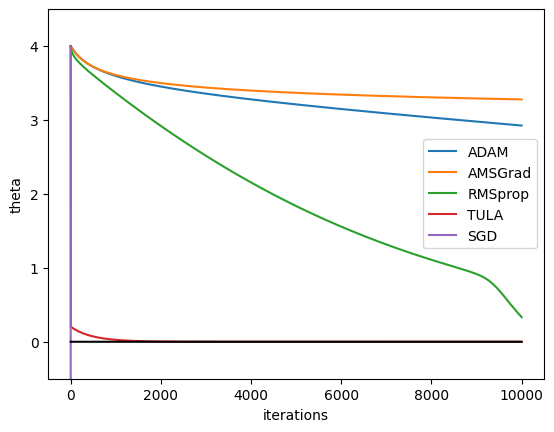
\includegraphics[width=0.5\linewidth]{image-wdTULA.png}
    \caption{Performance of different optimization algorithms}
    \label{fig:beta-opt}
\end{figure}
\end{document}
